% FA18 CSE 158 Assignment 2
% Sumeet Bansal and Subhankar Panda

\documentclass[11pt]{article}

%\usepackage[utf8]{inputenc} % set input encoding (not needed with XeLaTeX)

\usepackage{geometry}
\geometry{letterpaper}
\geometry{margin=0.8in}

\usepackage{graphicx}
\usepackage{svg}
\usepackage{hyperref}
\usepackage[parfill]{parskip}

\title{FA18 CSE 158 Assignment 2}
\author{Sumeet Bansal \& Subhankar Panda}

\begin{document}
\maketitle

\section{Dataset: NY Bus Breakdowns and Delays}
\subsection{Context}
The NYC Office of Pupil Transportation (OPT) provides transportation services to different locations, typically schools (public, private, or religious) but sometimes offices or other education-related sites within the limits of New York City or up to fifty miles from the city limits in bordering states New York, New Jersey, or Connecticut.

The NYC OPT's Bus Breakdown and Delay system is publicly accessible and collects information in real time from various contracted school bus vendors about any bus breakdowns or delays encountered. All system information is manually entered by school bus vendor staff. The primary dataset can be found \href{https://data.cityofnewyork.us/Transportation/Bus-Breakdown-and-Delays/ez4e-fazm}{\color{blue}here}.

We make use of a second, related dataset that contains more geographically-detailed information about the transportation sites tracked by OPT. That dataset can be found \href{https://data.cityofnewyork.us/Transportation/Transportation-Sites/hg3c-2jsy}{\color{blue}here} and is used only to complement the primary Bus Breakdowns and Delays dataset.

\subsection{Exploratory Analysis}

The dataset contains 254,247 data points and has the following schema:
\begin{table}
\begin{tabular}{ll}
\bf{Field} & \bf{Description} \\
School\_Year & Indicates the school year the incident occurred in. \\
Busbreakdown\_ID & Unique ID of each incident. \\
Run\_Type & Specific category of busing service. \\
Bus\_No & Bus number assigned by the bus vendor. \\
Route\_Number & Unique identifier of route taken. \\
Reason & Reason for breakdown or delay by reporting staff. \\
Schools\_Serviced & OPT codes of all transportation sites on the route. \\
Occurred\_On & Time/date of incident. \\
Created\_On & Time/date the record was logged by the OPT system. \\
Boro & Borough, county, or state in which the incident occurred. \\
Bus\_Company\_Name & Bus vendor name. \\
How\_Long\_Delayed & Length of delay as estimated by vendor staff. \\
Number\_Of\_Students\_On\_The\_Bus & Number of students on the bus during the incident. \\
\end{tabular}
\end{table}
\begin{table}
\begin{tabular}{ll}
\bf{Field} & \bf{Description} \\
Has\_Contractor\_Notified\_Schools & Indicator status as reported by vendor staff. \\
Has\_Contractor\_Notified\_Parents & Indicator status as reported by vendor staff. \\
Have\_You\_Alerted\_OPT & Indicator status as reported by vendor staff. \\
Informed\_On & Date on which the school, parents, or OPT was notified. \\
Incident\_Number & Reference for incidents reported to OPT Customer Service line. \\
Last\_Updated\_On & Time/date the record was last edited in the OPT system. \\
Breakdown\_or\_Running\_Late & Indicator status as reported by vendor staff. \\
School\_Age\_or\_PreK & Indicator of the population served by the route. \\
\end{tabular}
\end{table}

First, we remove irrelevant fields from the dataset, e.g. \texttt{Bus\_No} (not unique since many vendors might have a Bus \#1) , metadata (e.g. \texttt{Created\_On}, \texttt{Last\_Updated\_On}), and any post-breakdown/delay data (e.g. \texttt{Has\_Contractor\_Notified\_Schools}, \texttt{How\_Long\_Delayed}).

\subsubsection{\texttt{School\_Year}}
The \texttt{School\_Year} field indicates which school year a given incident occurred in.
\begin{center}
\includegraphics[width=5.25in]{images/school_year.png}
\end{center}
There is an upward trend, as more incidents occur each year from 2015 (the year the OPT system became operational) through present-day, which could be a result of steadily increasing traffic and population density, both of which would exacerbate delays and contribute to breakdowns. There is also a marked drop in 2018-2019 since that is the current school year and consequently incomplete.

\subsubsection{\texttt{Run\_Type}}
The \texttt{Run\_Type} field indicates which busing service the incident occurred during, e.g. General Ed AM Run is a ``stop-to-school service in the morning with pick-ups at bus stops and drop-offs at school(s)''---the traditional school bus service.
\begin{center}
\includegraphics[width=5.25in]{images/run_type.png}
\end{center}
By far, the most common type of busing service on which an incident occurs is the Special Ed AM Run (142,127 incidents), with the General Ed AM Run (33,928 incidents), Pre-K/EI (33,681 incidents), and Special Ed PM Run (34,033 incidents) services being the next common.

\subsubsection{\texttt{Reason}}
The \texttt{Reason} field indicates the exact reason why an incident occurs, e.g. heavy traffic would understandably cause a delay.
\begin{center}
\includegraphics[width=5.25in]{images/reason.png}
\end{center}
By far, the most common reason for an incident is heavy traffic---154,413 of the total 254,247 incidents---which makes sense in the denser, more urban areas of New York City, especially considering that NYC is the third most traffic-congested city in the world. Other common (named) reasons include mechanical problems (25,878 incidents), flat tires (7,732 incidents), and buses not starting (11,402 incidents), all of which are relatively common automobile issues.

\subsubsection{\texttt{Schools\_Serviced}}
The \texttt{Schools\_Serviced} field is a comma-separated list of the transportation sites that were to be serviced on the route on which the incident occurred. Pre-K/EI sites are denoted with one alpha, three numeric, and sometimes one additional alpha character. Otherwise, school-age sites are denoted with five numbers.
\begin{center}
\includegraphics[width=5.25in]{images/schools_serviced.png}
\end{center}
This box plot shows that the vast majority of sites have only had a few incidents over the past several years---approximately 7 per site (the median number of incidents)---but there are several sites that are very incident-prone, possibly due to poorly-maintained roads or traffic being especially congested in that area. If the high number of incidents in some sites is due to local factors, then many nearby sites must also see similarly high numbers of incidents regularly. So, many of these particularly incident-prone sites can be geographically clustered, where the high incidence rates of these clusters are products of the poor driving conditions in the area. To test this theory, we can visualize these geographic clusters with a heatmap, where hotter areas are indicative of poor driving conditions. The box plot above tells us that the median number of incidents is very low, but the outlying incident-prone sites skew the mean (of approximately 50) right. So, for each site, we normalize the number of incidents with the mean number of incidents and then filter the sites by those that have incidence rates greater than the mean, i.e. those that are more incident-prone. Then, with all the incidents in these sites' areas, we can graph a heatmap, thus visualizing the most incident-prone of these geographic clusters, where the hotter a cluster is, the more incidents occur in that cluster.

This visualization is where the secondary transportation site dataset came in handy, since it provided accurate geographical data for sites such as latitudes and longitudes, through which we can create a geographically-accurate heatmap.
\begin{center}
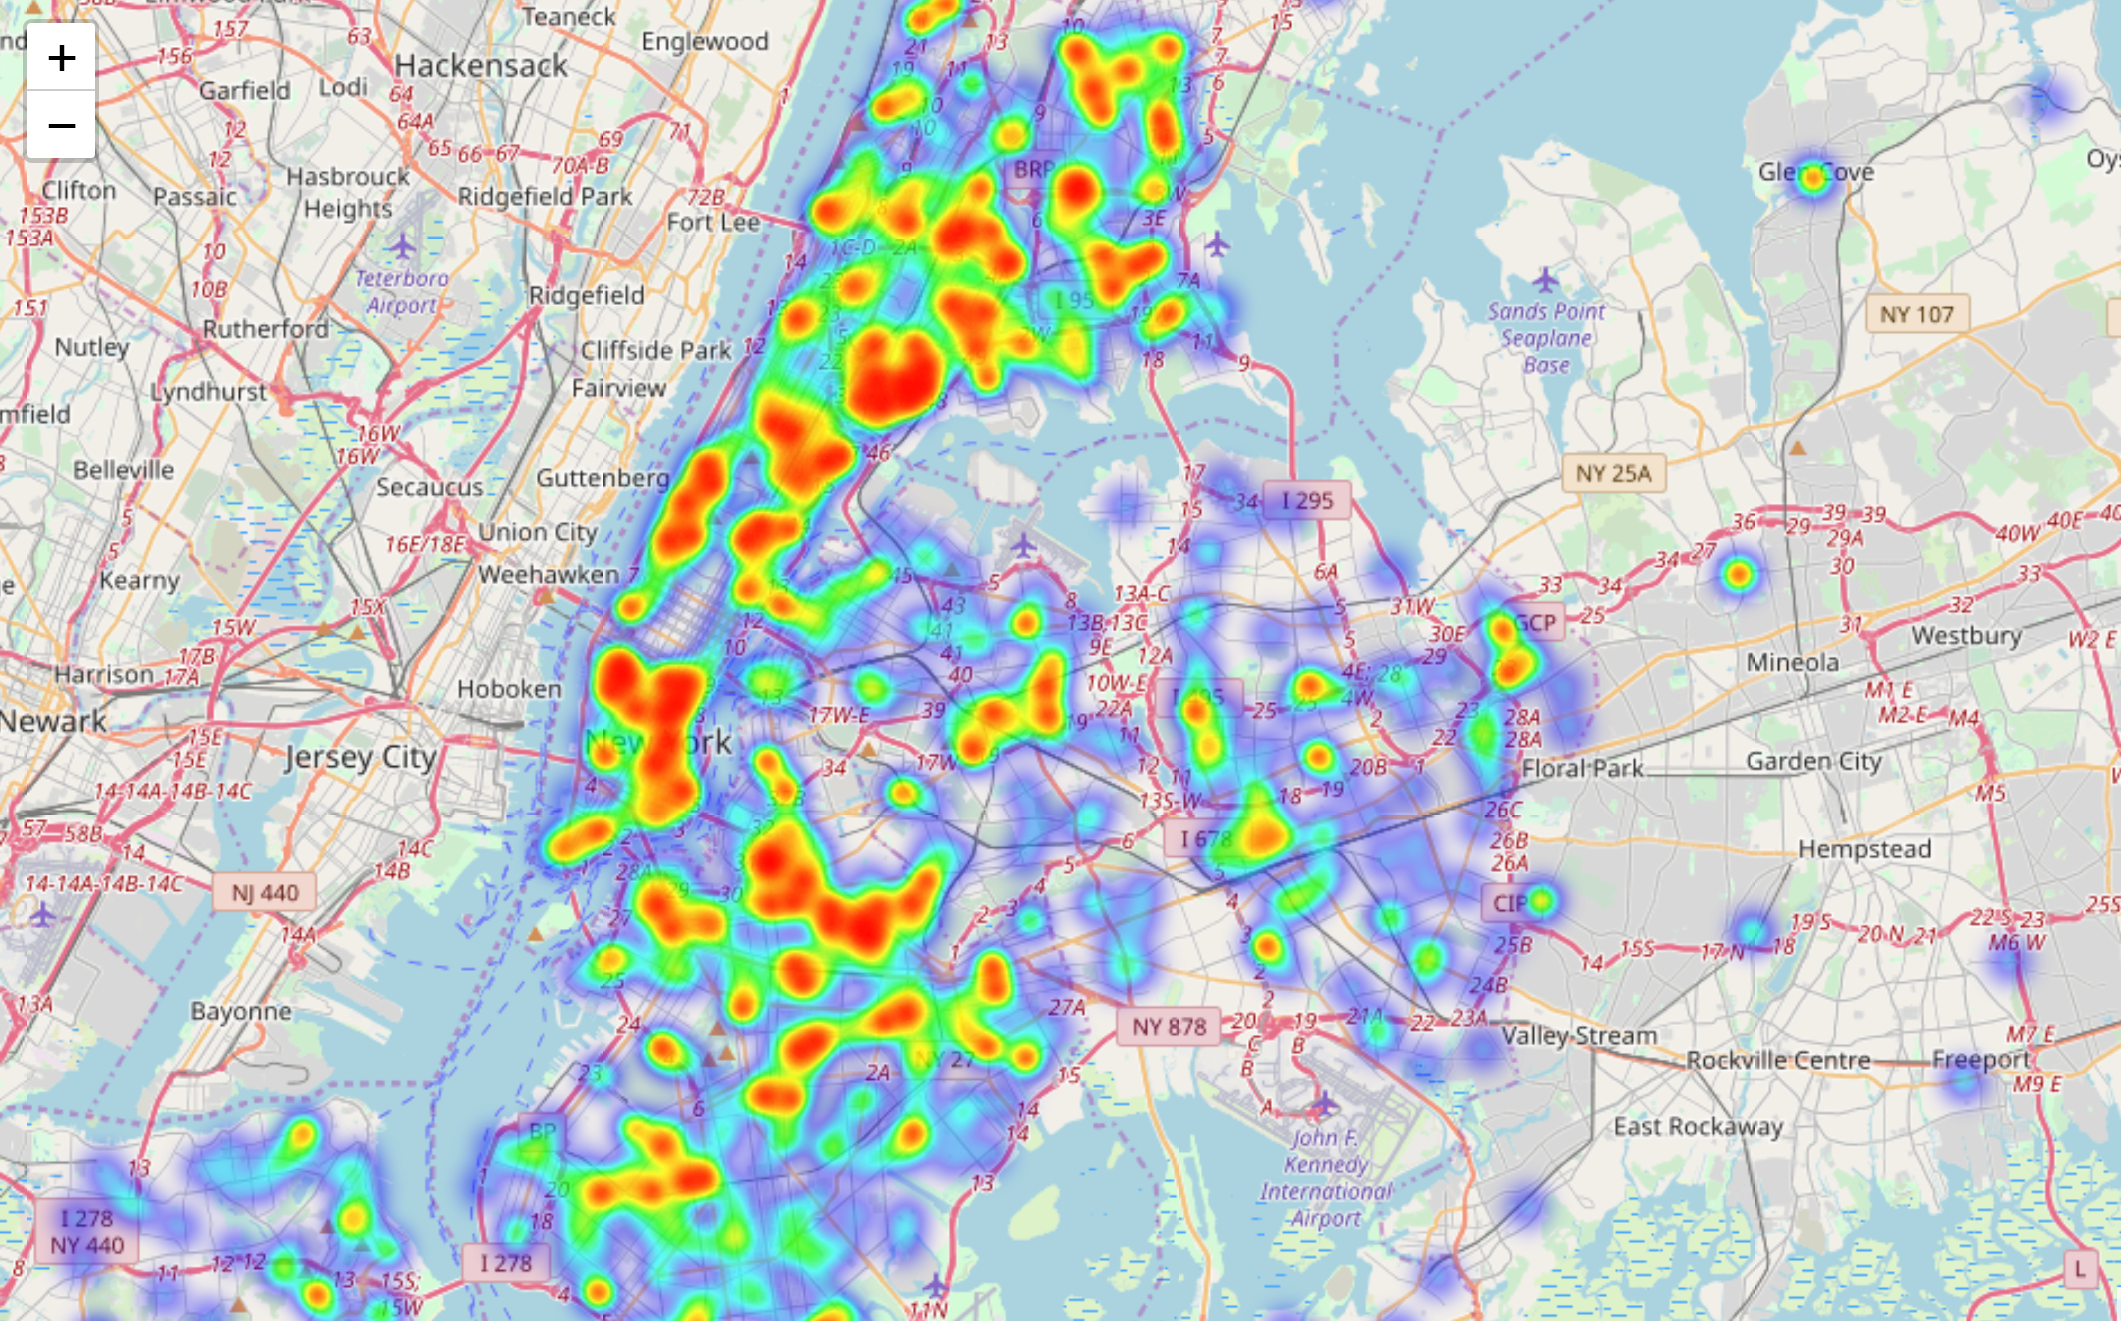
\includegraphics[width=6.9in]{images/heatmap.png}
\end{center}
This shows us that there are indeed certain geographic clusters where delays and breakdowns are especially common, such as the more densely populated areas of Manhattan (e.g. around Central Park, a prime tourist destination year-round), while also confirming that delays and breakdowns are much less common in the relatively suburban areas of New York City.

\subsubsection{\texttt{Occurred\_On}}
The \texttt{Occurred\_On} field indicates approximately when an incident occurred. We can parse this field as a \texttt{datetime} object and extract year, month, day, etc. Since the year of an incident is given more contextually accurately by the \texttt{School\_Year} field, analyzed earlier, and the day of the month of an incident isn't particularly useful, we look at the months, weekdays, and hours of incidents.

From the graphs on the next page, we can make a few observations. The number of incidents in the winter months are significantly higher than the number of incidents otherwise. However, this is likely the result of only having the incident data for the winter months of the 2018-2019 school year, inflating the number of incidents during these months relative to the other months. When accounting for this inflation, the number of incidents per month is relatively variable and no discernible pattern exists. The number of incidents per weekday is fairly stable, but there is a somewhat downward trend as the week progresses (from Monday to Friday). Finally, the number of incidents per hour spikes during the usual commuting hours (6-8 AM and 1-3 PM), as expected, although there is a significant reduction in the number of incidents when comparing the morning and afternoon hours. This reduction may the result of school letting out before most adults leave work, leading to less congested roads during the afternoon hours and fewer delays and breakdowns as a result.

\begin{center}
\includegraphics[width=4.25in]{images/month.png}
\includegraphics[width=4.25in]{images/weekday.png}
\includegraphics[width=4.25in]{images/hour.png}
\end{center}

\subsubsection{\texttt{Boro}}
The \texttt{Boro} field indicates the borough or county in which an incident occurred. The original data includes state data, but during data pre-processing, we removed incidents in Connecticut and New Jersey since we are considering incidents in New York alone.
\begin{center}
\includegraphics[width=5.25in]{images/boro.png}
\end{center}
The number of incidents for each borough/county can be split up into three tiers: high incidence rates, medium incidence rates, and low incidence rates. Unsurprisingly, the three most populous boroughs (Brooklyn, Manhattan, and Bronx) all belong in that first tier of high incidence rates, likely a result of the greater population density. Another borough, Queens, has the medium tier to itself, and the smaller counties (Nassau, Westchester, Staten Island, and Rockland) all have low incidence rates.

\subsubsection{\texttt{Bus\_Company\_Name}}
The \texttt{Bus\_Company\_Name} field indicates which bus vendor a broken-down or delayed bus belongs to.

On the next page, we can see that certain bus vendors have significantly greater numbers of incidents. These incident-prone vendors include, Leesel Transportation (35045 incidents), G.V.C. LTD. (23777 incidents), Pioneer Transportation (23335 incidents), and Reliant Transportation (20611 incidents). These incident numbers may either be the result of low bus quality or high usage rates (which would result in a high number of incidents, even at an average incidence rate).
\begin{center}
\includegraphics[width=5.25in]{images/bus_company_name.png}
\end{center}

\subsubsection{\texttt{Breakdown\_Or\_Running\_Late}}
The \texttt{Breakdown\_Or\_Running\_Late} field indicates whether an incident is the result of a breakdown or a delay.
\begin{center}
\includegraphics[width=5.25in]{images/breakdown_vs_delay.png}
\end{center}
There are significantly more delays (225,343 incidents) than there are breakdowns (28,904 incidents), which makes sense considering the heavy traffic of the area.

\subsubsection{\texttt{School\_Age\_or\_PreK}}
The \texttt{School\_Age\_or\_PreK} field indicates whether an incident occurred on a bus carrying school-age or Pre-K/EI children.
\begin{center}
\includegraphics[width=5.25in]{images/school_type.png}
\end{center}
There are significantly more incidents involving school-age chidren (220,566 incidents) than there are involving Pre-K/EI children (33,681 incidents), likely because there are many more school-age children and therefore more school-age bus services than there are Pre-K/EI children and Pre-K/EI bus services.

\newpage
\section{Predictive Task: Breakdowns vs. Delays}	
For our predictive task, we will classify an incident as either a breakdown or a delay. To do this, we will divide the dataset into training and validation sets and evaluate the model by its accuracy on the validation set. Since the majority of incidents are classified as delays, our baseline will be a trivial predictor that always classifies incidents as breakdowns; this should have an accuracy of approximately 88.6\% since that is the ratio of total breakdowns to total incidents.

\subsection{Features}
Of the features explored in the section above, we want to find the most promising for a binary classifier; these features will typically be ones where the ratio of breakdowns to delays for any given category is significantly different from the ratio of total breakdowns to total delays, indicating that that certain values of that category are more likely to come from either a breakdown or a delay. By combining several of these differentiating features, we can build a binary classifier that distinguishes between breakdowns and delays fairly accurately. The ratio of total delays to total breakdowns is approximately 7.8.

\subsubsection{\texttt{Run\_Type}}
The first feature we consider using in our model is \texttt{Run\_Type}.
\begin{center}
\includegraphics[width=5.25in]{images/run_type_stacked.png}
\end{center}
We see that some categories in \texttt{Run\_Type} tend to have more delays than usual and some tend to have more breakdowns than usual; for example, the ratio of total delays to total breakdowns is approximately 7.8 but the ratio for Special Ed AM Run is 9.4 and the ratio for Pre-K/EI is 49.4, indicating that these incidents are more likely to be delays than usual. This significant different for Pre-K/EI incidents could possibly be due to bus services for younger children being much safer than bus services for school-age children, leading to significantly fewer breakdowns. Therefore, \texttt{Run\_Type} categories make good candidates for feature representations.

\subsubsection{\texttt{Reason}}
The next feature we consider using in our model is \texttt{Reason}.
\begin{center}
\includegraphics[width=5.25in]{images/reason_stacked.png}    
\end{center}
Reasons directly correlate to incident classification, e.g. heavy traffic leads to delays. This direct correlation is displayed by the stacked bar chart above, where Heavy Traffic has a delay to breakdown ratio (explained in the subsection above) of 403.2---if an incident has Heavy Traffic listed as its reason, it is almost invariably a delay and not a breakdown--while Mechanical Problem has a ratio of 0.86, so an incident with Mechanical Problem listed as its reason is much more likely to be a breakdown than usual. Therefore, \texttt{Reason} categories make excellent candidates for feature representations.

\subsubsection{\texttt{Schools\_Serviced}}
The next feature we consider using in our model is \texttt{Schools\_Serviced} using the same heatmap visualizations mentioned in our exploratory analysis.
\begin{center}
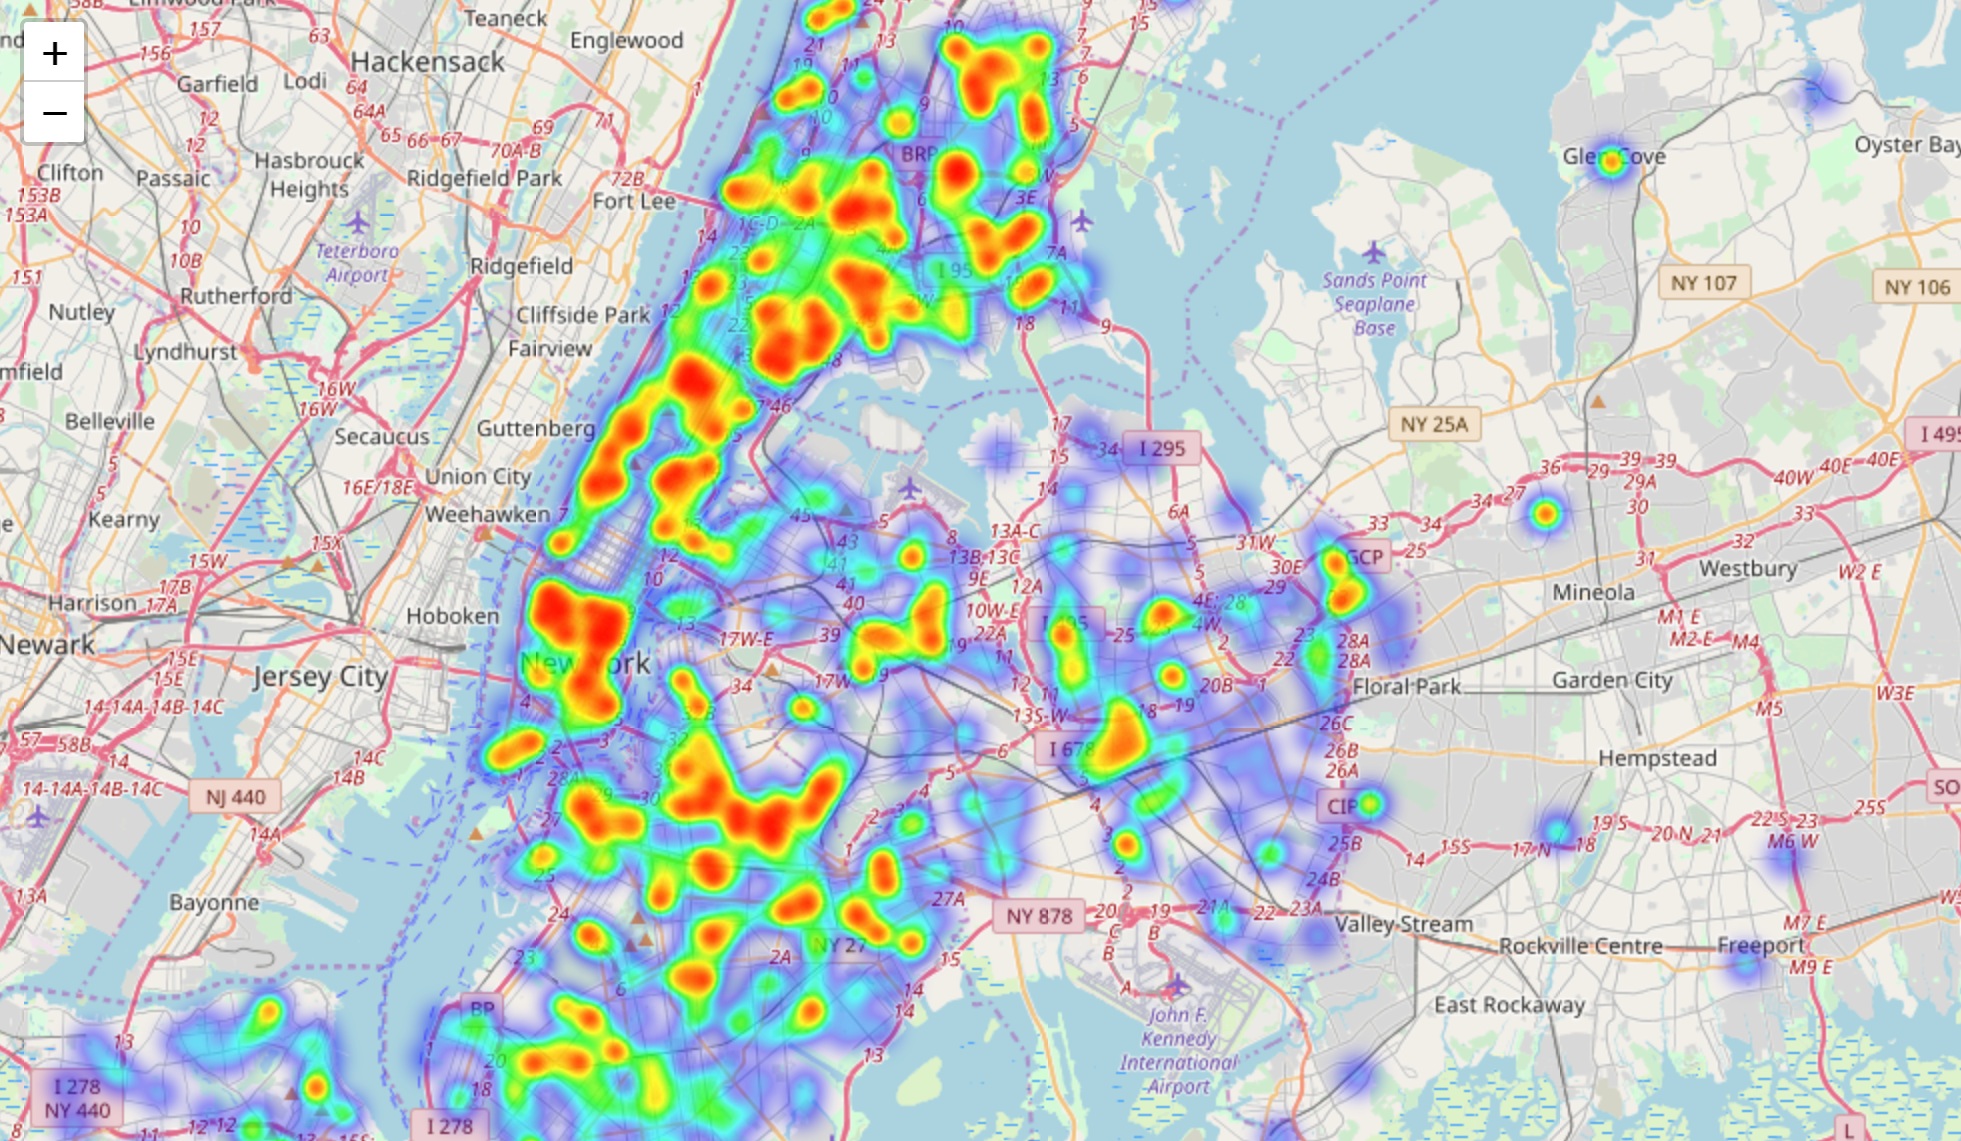
\includegraphics[width=3.4in]{images/heatmap_breakdown.png}    
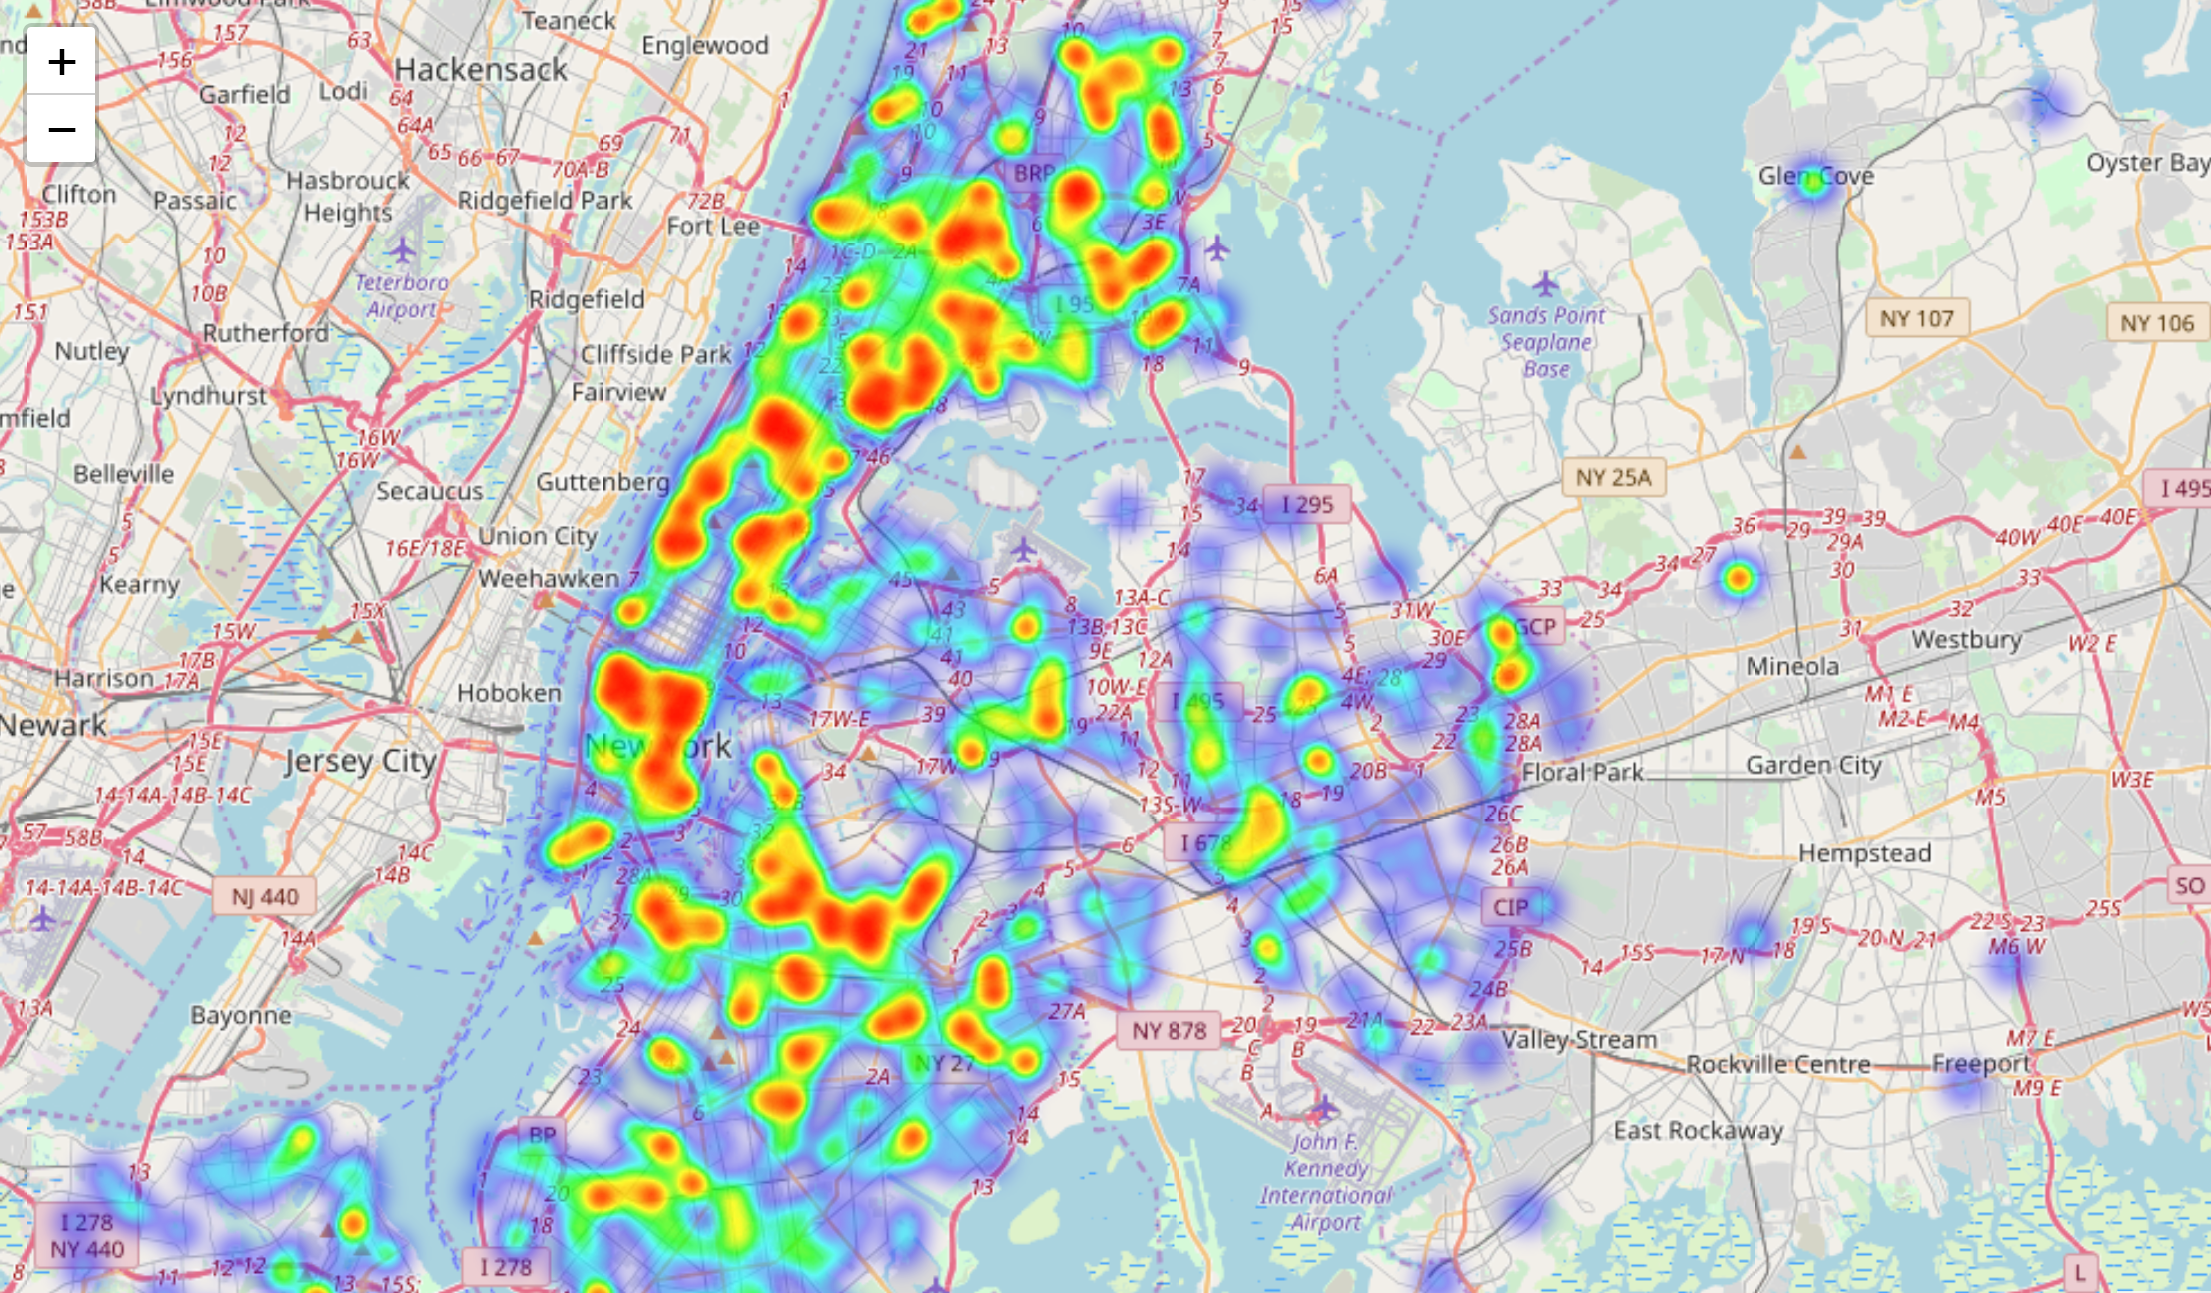
\includegraphics[width=3.4in]{images/heatmap_delay.png}    
\end{center}
Above are the heatmaps for exclusively breakdowns (left) and exclusive delays (right). Unfortunately, the heatmaps are fairly similar, and the greater radii of hot areas in the delays heatmap could be attributed to the greater number of data points for delays.

\subsubsection{\texttt{Occurred\_On}}
As explained earlier, we can parse this field's value into a \texttt{datetime} object for each data point, from which we can plot the following graphs.
\begin{center}
\includegraphics[width=4.5in]{images/month_stacked.png}
\includegraphics[width=4.5in]{images/weekday_stacked.png}
\end{center}
We can see that the months and weekdays above follow the general ratio of delays to breakdowns. However, the hours do not; some of the hours heavily tend to have more delays than usual or breakdowns than usual. For example, 7-8 AM has a ratio of 15.0---well above the typical ratio--and 8-9 AM, the following hour, has an even higher ratio of 17.8, which makes sense considering those hours are prime commuting hours in the morning. So, while the month and weekday would not be effective features, the hour of an incident might be.
\begin{center}
\includegraphics[width=5.25in]{images/hour_stacked.png}
\end{center}

\subsubsection{\texttt{Boro}}
The next feature we consider using in our model is \texttt{Boro}.
\begin{center}
\includegraphics[width=5.25in]{images/boro_stacked.png}
\end{center}
Again, we see that some boroughs and counties tend to have more breakdowns or delays than usual: Nassau County has a ratio of 4.9, Manhattan 18.9, Queens 3.2, Westchester 49.5, Staten Island 29.6, and Bronx 6.7. Nassau County, Queens, and Bronx all tend to have significantly more breakdowns than usual, whereas Manhattan, Westchester, and Staten Island all tend to have significantly more delays than usual. Unsurprisingly, Manhattan and Staten Island are both tourist destinations that experience severe traffic. The high variances of the boroughs and counties make them excellent predictors of whether an incident is a breakdown or a delay, and although the geographic clustering method (using heatmaps) did not quite pan out, this is a suitable substitute for more granular geographic clustering.

\subsubsection{Bus\_Company\_Name}
The next feature we consider using in our model is \texttt{Bus\_Company\_Name}.
\begin{center}
\includegraphics[width=5.25in]{images/bus_company_name_stacked.png}
\end{center}
Some bus vendors have significantly higher rates of breakdowns than usual, such as Little Ritchie Bus Service (0.99), Logan Bus Company (1.37), and the unreliable Reliant Transportation (6.6), and some bus vendors have significantly lower, i.e. safer, rates of breakdowns than usual, such as Pioneer Transportation (1665.8), Leesel Transportation (85.7), and G.V.C. Ltd. (60.1). Therefore, bus vendors make for great features as well.

\subsubsection{\texttt{School\_Age\_or\_PreK}}
The final feature we consider using in our model is \texttt{School\_Age\_or\_PreK}.
\begin{center}
\includegraphics[width=5.25in]{images/school_type_stacked.png}
\end{center}
As we can see, there's a significant difference in the delay to breakdown ratio for school-age (6.8) and pre-k children (494), making the kind of school serviced a good feature for our model as well.

\subsection{Good Features}
To summarize, the features that we believe will be useful in differentiating are \texttt{Run\_Type}, \texttt{Reason}, \texttt{Occurred\_On} (but only the hours, not the weekdays, months, or anything else), \texttt{Boro}, \texttt{Bus\_Company\_Name}, and \texttt{School\_Age\_or\_PreK}.

\newpage
\section{A Binary Classifier}

From our exploratory analysis and stacked bar graphs, we were quickly able to see that the ratio between Delays and Breakdowns was very high for certain data points like \texttt{Run\_Type}, \texttt{Reason}, \texttt{Occurred\_On} (but only the hours, not the weekdays, months, or anything else), \texttt{Boro}, \texttt{Bus\_Company\_Name}, and \texttt{School\_Age\_or\_PreK}. Because of the discrepancy between Breakdowns and Delays for these data points, they are good data points to model our feature around. 

\subsection{\texttt{Linear Regression}}

We started out with a classic linear regression classifier and modeled a basic starter predictor, where our features included all 6 variables we identified as good distinguishing characteristics. To evaluate this predictor, we used the \texttt{r-squared} metric on a scale of 0 to 1, where 1 indicates a perfectly fitting model. On our initial model, we calculated an \texttt{r-squared} value of $R^2=0.42$, which was not even as performant as our baseline. Modified versions of this model using different feature combinations were not promising either.

At this point we were fairly surprised by the underwhelming linear regression performance. We soon realized that we were modeling a linear regressor on categorical data, instead of continuous data. Linear regressors estimate parameters by minimizing the sum of the squared errors (SSE). This approach does not work for categorical data because it is by definition not continuous, so the SSE is not a very valid metric for prediction. We realized that predicting by the actual likelihood was not working out too well either, so we moved on to another model that made predictions by minimizing the training error, i.e. an SVM.

\subsection{\texttt{SVM}}

Our next approach was to use an SVM as our model. Using the same feature representations as above, we ran a starter test on the data. With all the variables added to the feature, we achieved an accuracy of 90.2\% on the validation set, an incredible jump in performance from the linear regressor and an improvement on our baseline.

After playing around with the features a little more, we were still unable to beat the 90.2\% validation accuracy we had just achieved. With the 6 features we had identified as suitable for this predictive task, we realized we had $2^6=64$ possible feature combinations, and finding a better model by randomly testing features would not be nearly as effect as programmatically generating each of these 64 possible models and validate their accuracies. Then, sorting by validation accuracy yielded us our optimal models using an SVM. These optimal models are listed below.

\begin{table}[h]
\centering
\begin{tabular}{cccccc|cc}
\bf{Reason} & \bf{Service} & \bf{Boro} & \bf{Age} & \bf{Hours} & \bf{Vendor}& \bf{Training} & \bf{Validation} \\
True & True & True & False & False & True & 0.9448 & 0.9417 \\
True & True & True & False & True & True & 0.9448 & 0.9417 \\
True & True & True & True & False & True & 0.9448 & 0.9417 \\
True & True & True & True & True & True & 0.9448 & 0.9417 \\
\end{tabular}
\end{table}

However, upon closer examination of the data, we realized that the conditions for some breakdowns closely matched the conditions for some delays, and the SVM would prioritize classifying these difficult data points instead of taking into account how highly imbalanced the data is. Since an SVM would be more inaccurate because of this imbalance, we tried a third model: logistic regression.

\subsection{\texttt{Logistic Regression}}
As we previously identified, there were 6 features that were suitable for classifying incidents as breakdowns and delays: \texttt{Run\_Type}, \texttt{Reason}, \texttt{Occurred\_On} (but only the hours, not the weekdays, months, or anything else), \texttt{Boro}, \texttt{Bus\_Company\_Name}, and \texttt{School\_Age\_or\_PreK}. Again, with many features in play, it was difficult to intuitively find the best combination of features out of the possible 64 configurations to maximize our model's accuracy, so we programmatically generated and validated each of these models, thus yielding the following optimal models.

\begin{table}[h]
\centering
\begin{tabular}{cccccc|cc}
\bf{Reason} & \bf{Service} & \bf{Boro} & \bf{Age} & \bf{Hours} & \bf{Vendor} & \bf{Training} & \bf{Validation} \\
True & True & True & False & False & True & 0.9446 & 0.9424 \\
True & True & True & False & True & True & 0.9446 & 0.9424 \\
True & True & True & True & False & True & 0.9446 & 0.9424 \\
True & True & True & True & True & True & 0.9446 & 0.9424 \\
\end{tabular}
\end{table}

We can see that the feature combinations for the optimal SVMs and optimal logistic regressors are exactly the same, verifying for us that these feature combinations are the most optimal for prediction.

The 94.24\% accuracy is a respectable performance jump from the SVM. As expected, the logistic regressor was more accurate than the SVM, if only by 0.02\%, because it takes into account the data imbalance instead of minimizing the classification error and incorrectly prioritizing the difficult data points where the conditions for a breakdown is similar to the typical conditions for delays, vice versa, since this would lead to a less optimal classifier that isn't as confident for certain data points as it could be if it ignored these outlying data points.

\newpage
\section{Related Literature}
This assignment uses data compiled by the NYC Open Data Project and stitches together 2 different datasets---NYC Bus Breakdown and Delay and NYC Transportation Sites---both of which were sourced directly from \href{https://opendata.cityofnewyork.us/}{\color{blue}the NYC Open Data Project's website}. We initially started with just the NYC Bus Breakdown and Delay dataset but soon realized that the approaches we wanted to explore would involve having more metadata about the routes and transportation sites than given to us. After finding the Sites dataset, we were able to link the two by using the unique Office of Pupils Transportation (OPT) code assigned to each site.

While browsing datasets on Kaggle, we often came across city-based service data. We looked at \href{https://www.kaggle.com/stoney71/new-york-city-transport-statistics}{\color{blue}the NYC Bus Dataset} and other large city transit data. We eventually decided to use our dataset to further investigate how geographical location, clientele type, employees and other seemingly unrelated data points correlated to bus breakdowns. On further research of this data set, we found \href{https://datascienceplus.com/nyc-bus-delays/}{\color{blue}this amazing blog post} on datascienceplus.com, which does a exploratory data visualization analysis of our dataset. This blog post gave us an early glimpse into the kind of data we were dealing with, helping us spot trends like the massive bias towards Delays over Breakdowns early. The post let us hit the ground running and gave us a good foundation to ideate upon. This also inspired us to have a data visualization centered approach to our exploration, which was very helpful in giving us an intuitive understanding of our subject data.

While investigating this dataset we mostly employed data science techniques learned in this course but were often thrown off track by trying to employ a new technique that we read on a blog post. A few examples of this include us toying with the idea of building a \href{https://machinelearningmastery.com/implement-perceptron-algorithm-scratch-python/}{\color{blue}Perceptron Binary Classifier} or a \href{https://arxiv.org/pdf/1509.03891v1.pdf}{\color{blue}Convolutional Neural Network}. While these techniques were definitely exciting, we held off on implementing them into our project in the interest of time. Other abandoned approaches include geographic clustering (visualized as heatmaps), for which we used a number of methods, such as the clustering algorithms described in \href{https://towardsdatascience.com/the-5-clustering-algorithms-data-scientists-need-to-know-a36d136ef68}{\color{blue}this blog post} and the \texttt{networkx} libraries for \href{https://networkx.github.io/documentation/stable/reference/algorithms/clustering.html}{\color{blue}clustering} and \href{https://networkx.github.io/documentation/networkx-1.10/reference/algorithms.component.html}{\color{blue}components}, before we realized that that cluster data would not be useful since areas with abnormally high delays were also areas with abnormally high breakdowns and it would not be feasible to implement geographic clustering in a model.

Another cool project we learned a lot from is \href{http://cs229.stanford.edu/proj2016/report/Nissimoff-RealTimeLearningAndPredictionOfPublicTransitBusArrivalTimes-report.pdf}{\color{blue}this Stanford CS229 Project} where the author uses the same idea of geographic clustering by latitude and longitude to predict public transit delays. This project has access to significantly more data than ours and is a mathematical deep dive into the current technologies that can be used to solve this problem. An interesting idea that this paper proposes is the use of "Route-Segments": bus routes are usually long and involve going through a lot of diverse terrains, which is definitely a factor in the frequency of breakdowns, so it makes sense to think of route segments as local minima and maxima to mathematically quantify the road quality of the segments' surrounding areas.

We learned in our research that the techniques we were using (linear regression, logistical regression, SVMs, etc.) were not too far from the methods used in industry to solve similar problems. In industry, companies are definitely using newer, hotter technologies like deep/reinforcement learning, but our 94.2\% validation set accuracy shows that the tried and tested methods are still highly functional.

\newpage
\section{Results and Conclusion}
In order to determine the most optimal combination of feature representations for our model, we trained and validated a logistic regressor using every possible combination of feature representations ($2^6=64$ combinations), and the results of these runs are shown below, sorted by accuracy on a (consistent) validation set. Since many models had the same training and validation accuracy, all models that achieved a top 3 validation accuracy are listed, and at least one model for the remaining accuracies is listed.

\begin{table}[h]
\centering
\begin{tabular}{cccccc|cc}
\bf{Reason} & \bf{Service} & \bf{Boro} & \bf{Age} & \bf{Hours} & \bf{Vendor} & \bf{Training} & \bf{Validation} \\
True & True & True & False & False & True & 0.9446 & 0.9424 \\
True & True & True & False & True & True & 0.9446 & 0.9424 \\
True & True & True & True & False & True & 0.9446 & 0.9424 \\
True & True & True & True & True & True & 0.9446 & 0.9424 \\
True & True & False & False & False & True & 0.9447 & 0.9395 \\
True & True & False & False & True & True & 0.9447 & 0.9395 \\
True & True & False & True & False & True & 0.9447 & 0.9395 \\
True & True & False & True & True & True & 0.9447 & 0.9395 \\
False & True & False & False & False & True & 0.9433 & 0.9391 \\
False & True & False & False & True & True & 0.9433 & 0.9391 \\
False & True & False & True & False & True & 0.9433 & 0.9391 \\
False & True & False & True & True & True & 0.9433 & 0.9391 \\
False & True & True & False & False & True & 0.9430 & 0.9388 \\
True & True & True & False & False & False & 0.9247 & 0.9243 \\
False & True & True & False & False & False & 0.9208 & 0.9182 \\
True & True & False & False & False & False & 0.9103 & 0.9072 \\
False & True & False & False & False & False & 0.9106 & 0.9029 \\
False & False & True & False & False & True & 0.8891 & 0.8995 \\
True & False & False & False & False & True & 0.8940 & 0.8941 \\
False & False & False & False & False & True & 0.8848 & 0.8940 \\
True & False & True & False & False & True & 0.8940 & 0.8939 \\
False & False & False & False & False & False & 0.8820 & 0.8914 \\
\end{tabular}
\end{table}

The most accurate models we created all have a training accuracy of 0.9446 and a validation accuracy of 0.9424, 5\% higher than our baseline and generally extremely accurate. Our most accurate alternate model, an SVM trained on the same feature representations, had a training accuracy of 0.9448 and a validation accuracy of 0.9417--a marginally higher training accuracy but lower validation accuracy, indicating that the SVM was overfitting slightly more than the logistic regressor.

We can see that Reason (\texttt{Reason}), Service (\texttt{Run\_Type}), Boro (\texttt{Boro}), and Vendor (\texttt{Bus\_Company\_Name}) are used as features in every version of the optimal model, which follows our claim that those two would be the most useful features, but Service and Vendor are used as features in every model with a top 3 accuracy (the top 12 models), which is interesting because we identified Reason as the most valuable feature due to its categories' very direct correlations to breakdowns and delays (e.g. Heavy Traffic).

The features for Age (\texttt{School\_Age\_or\_PreK}), and Hours (derived from \texttt{Occurred\_On}) are used in some optimal models, but there doesn't seem to be a discernible pattern to their usages.

Our baseline---a trivial predictor that always returns "Delay" (the overwhelming majority of incident classifications)---ranks dead last and interestingly performs better on the validation set than it does on the training set, indicating that the training set contains slightly more delays than expected, but the validation set had a balanced ratio of delays and breakdowns.

Our final model would therefore be using a feature representation of Reason, Service, Boro, and Vendor, which takes into account the reason for an incident, what type of bus service it occurred on, approximately where geographically it occurred, and the vendor of the bus involved in the incident, since all optimal models used those four features, and other features (i.e. Age and/or Hours) did not make a difference in the final accuracy of a model, so including those features would result in a somewhat less time- and space- efficient model.

Despite the already high baseline, this final model likely succeeded due to the relevancy of its features: Reason directly correlates to the incident classification, Service takes into account how bus quality per service affects incident classification (e.g. safer buses might be used to transport younger children or the buses for more common services might see significantly more wear-and-tear than usual, leading to more breakdowns), Boro most directly represents the heavy traffic that causes the majority of incidents/delays in the more densely populated areas of New York City, and Vendor serves as an indirect factor for bus quality since different vendors purchase safer buses for various clients or might service exclusively service more urban routes (which are more likely to experience delays).

\end{document}

